% µFlow: Advances in Engineering Software (Elsevier, ISSN 0965-9978)
% Submitted March 2026
% =====================================================================
\documentclass[preprint,review,12pt]{elsarticle}

\usepackage{lineno}
\modulolinenumbers[5]
\usepackage{hyperref}
\usepackage{graphicx}
\usepackage{amsmath,amssymb}
\usepackage{booktabs}
\usepackage{multirow}
\usepackage{array}
\usepackage{url}
\usepackage{xcolor}
\usepackage{siunitx}
\usepackage{enumitem}
\usepackage{float}

\sisetup{
  per-mode=symbol,
  inter-unit-product=\ensuremath{\cdot},
  range-phrase=--,
  range-units=single
}
\DeclareSIUnit\decibel{dB}
\DeclareSIUnit\minute{min}
\DeclareSIUnit\hour{h}
\DeclareSIUnit\day{d}

\journal{Advances in Engineering Software}

% =====================================================================
% HIGHLIGHTS (required by AIES, max 85 chars each, 3--5 bullets)
% Include as comment block; also submit separately via EES
% =====================================================================
% Highlights:
% - Browser-based 3D simulator for microfluidic Hall-effect bead detection
% - Four coupled physics modules validated against FEM-BEM benchmarks
% - 12 sensor materials and 8 bead presets from peer-reviewed data
% - Parametric sweep engine computes 1000 configurations in seconds
% - Built-in 2D axisymmetric FEM solver validates the analytical model
% =====================================================================

\begin{document}

\begin{frontmatter}

\title{$\mu$Flow: A Browser-Based Interactive Simulator for Microfluidic Hall-Effect Magnetic Bead Detection with Parametric Design Optimization}

\author[rutgers]{Harshitha Govindaraju\corref{cor1}}
\ead{harshitha.govindaraju@rutgers.edu}
\author[rutgers]{Umer Hassan}
\ead{umer.hassan@rutgers.edu}
\cortext[cor1]{Corresponding author. Tel.: +1-848-xxx-xxxx}
\affiliation[rutgers]{organization={Department of Electrical and Computer Engineering, Rutgers, The State University of New Jersey},
            addressline={94 Brett Road},
            city={Piscataway},
            postcode={08854},
            state={NJ},
            country={USA}}

\begin{abstract}
We present $\mu$Flow, an open-source, browser-based simulator that models the complete signal chain of microfluidic Hall-effect magnetic bead detection in an interactive three-dimensional environment. The tool implements four coupled analytical physics modules: Clausius--Mossotti bead magnetization, point-dipole stray-field computation, volume-averaged Hall voltage generation over an arbitrary sensor geometry, and Poiseuille microfluidic transport with optional magnetophoretic drift. A built-in material database provides 12 Hall sensor platforms, including graphene, III--V semiconductor heterostructures, Si CMOS, bismuth, and topological insulators, with gate-tunable carrier density for two-dimensional materials. All material parameters are drawn from peer-reviewed experimental data. $\mu$Flow reproduces finite-element method (FEM) benchmarks from our companion COMSOL study to within \SI{6}{\percent} relative error for three sensor designs spanning \SIrange{5}{50}{\micro\meter}, and includes a built-in 2D axisymmetric FEM magnetostatic solver that independently validates the analytical dipole model against a full volumetric field solution. A parametric sweep engine evaluates sensor geometry, material selection, flow velocity, and bead properties across thousands of configurations in seconds. The entire application is a single HTML file (${\sim}$\num{3000} lines) built on React~18 and Three.js, requiring no installation, no server, and no license. $\mu$Flow is deployed at \url{https://microfluidic-hall-sensor.vercel.app} and released under the MIT license.
\end{abstract}

\begin{keyword}
microfluidic simulation \sep Hall effect sensor \sep magnetic bead detection \sep parametric optimization \sep browser-based visualization \sep open-source software \sep biosensor design
\end{keyword}

\end{frontmatter}

\linenumbers

% ========================================================================
\section{Introduction}
\label{sec:intro}
% ========================================================================

Microfluidic Hall-effect sensors detect individual superparamagnetic beads by measuring the transient stray magnetic field as labeled analytes flow past a thin-film Hall element embedded in a microchannel floor. Ejsing et al.\ measured a \SI{0.3}{\micro\volt} signal change from a single \SI{2}{\micro\meter} bead using a planar Hall effect sensor magnetized at \SI{20}{\milli\tesla}, with the bipolar voltage transient providing both detection and position information as the bead traversed the sensor cross \cite{ejsing2004}. Shah et al.\ integrated CVD graphene Hall sensors with current-related sensitivity $S_I = \SI{175}{\volt\per\ampere\per\tesla}$ into a \SI{50}{\micro\meter} PDMS microchannel and detected \SI{47}{\micro\meter} ferrite-agarose beads in whole blood with SNR $> \SI{20}{\decibel}$; the graphene sensor maintained linear response over a \SI{100}{\milli\tesla} field range without observable drift during continuous flow operation \cite{shah2023}. Aledealat et al.\ tracked individual \SI{2.8}{\micro\meter} Dynabeads in real time using an InAs quantum-well micro-Hall sensor, observing that the sign-resolved voltage transient reversed polarity as beads entered and exited the active Hall cross, which they used to extract bead velocity from the pulse width \cite{aledealat2009}. Gabureac et al.\ resolved a single \SI{1}{\micro\meter} bead and traced its lateral position across the sensor area using a \SI{500}{\nano\meter} nanocomposite Hall sensor fabricated by focused electron beam-induced deposition \cite{gabureac2013}.

Graphene has become particularly attractive for Hall sensing because its low carrier density and high mobility yield large Hall coefficients at room temperature. Dauber et al.\ achieved a minimum detectable field of \SI{50}{\nano\tesla\per\sqrt{\hertz}} at room temperature using graphene encapsulated in hexagonal boron nitride, with the encapsulation reducing charge puddle disorder and suppressing $1/f$ noise by a factor of 10 relative to graphene on SiO$_2$ \cite{dauber2015}. Kaidarova et al.\ demonstrated a flexible Hall sensor from laser-scribed graphene on polyimide with a sensitivity of \SI{0.097}{\volt\per\volt\per\tesla} that survived bending to a \SI{4}{\milli\meter} radius over 1000 cycles without measurable degradation \cite{kaidarova2021}. These advances have broadened the landscape of candidate sensor materials, but selecting the optimal platform for a given bead, channel, and magnet configuration remains nontrivial because the detected signal depends on the coupled interaction of at least four physics domains.

The design challenge arises because: (a)~the magnetization of the bead in the applied field depends on its ferrite content and effective susceptibility through the Clausius--Mossotti relation; (b)~the spatial distribution of the bead's dipolar stray field decays as $1/r^3$ and changes sign at lateral offsets; (c)~the Hall voltage is produced by averaging this inhomogeneous field over the sensor active volume, so the signal depends jointly on bead size and sensor footprint; and (d)~the hydrodynamic transport determines the bead trajectory and transit time through the sensing zone via the Poiseuille velocity profile. Commercial finite-element tools such as COMSOL Multiphysics can model each of these domains, but setting up a coupled magnetostatic-hydrodynamic simulation requires a software license (typically \$3{,}000--\$8{,}000 per year) and hours of computation per parameter sweep. Our companion study used a COMSOL FEM-BEM model to compare three sensor geometries and four semiconductor platforms, requiring over 200 individual simulations \cite{govindaraju2025}. Jebari et al.\ reported that their 3D multiphysics simulation of a microfluidic immunosensor required coupled Navier--Stokes, convection-diffusion, and magnetostatic solvers across multiple geometry variants, each taking tens of minutes per configuration \cite{jebari2024}. No open-source, interactive alternative existed for rapid exploration of this design space.

$\mu$Flow addresses this gap. It is a publicly available simulator that integrates all four physics domains into a real-time, browser-based, three-dimensional visualization with a parametric sweep engine for automated design optimization and a built-in FEM solver for independent model validation. The tool targets three user communities: researchers exploring Hall sensor design trade-offs before committing to fabrication, educators teaching biosensor physics in courses where commercial FEM licenses are unavailable, and students learning the interplay of magnetic, electronic, and fluidic phenomena in lab-on-chip systems. Lab-on-chip platforms are under active development for point-of-care diagnostics \cite{tymm2020,coarsey2019,kabir2020}, and magnetic bead-based immunoassays in microfluidic channels have been demonstrated for both sandwich ELISA \cite{bhalla2013} and pathogen detection \cite{kabir2020}. A freely accessible simulation tool can accelerate sensor design iterations for these applications.

The contributions of this paper are:
\begin{itemize}[nosep]
\item A validated analytical model coupling bead magnetization, stray-field computation, volume-averaged Hall voltage, and Poiseuille transport, parameterized by a 12-material, 8-bead database drawn from published experimental data, with gate-tunable carrier density for two-dimensional sensor materials.
\item A browser-native software architecture (React~18, Three.js, HTML5 Canvas) that achieves real-time 3D visualization and signal computation with zero installation overhead, organized across six dedicated application pages.
\item A parametric sweep engine that evaluates thousands of sensor-bead-flow configurations in seconds, enabling automated identification of optimal operating points with CSV data export.
\item A 2D axisymmetric FEM magnetostatic solver implemented entirely in JavaScript, providing in-browser validation of the point-dipole approximation against a full volumetric field solution with adaptive mesh refinement, preconditioned conjugate gradient iteration, and interactive field visualization.
\item Quantitative validation against FEM-BEM simulations \cite{govindaraju2025} and published experimental data, with relative errors below \SI{6}{\percent} for all three benchmark designs.
\end{itemize}

Table~\ref{tab:comparison} compares $\mu$Flow against available alternatives. The MMFT simulator \cite{emmerich2024} models microfluidic networks using a 1D hydraulic-circuit analogy but does not include magnetic sensing. The nanoHUB BioSensorLab \cite{nanohub} models electrostatic FET-based biosensors rather than magnetic bead detection. Gurvich and Geller developed Firefly, a browser-based Three.js tool for interactive 3D visualization of datasets containing up to $10^7$ points \cite{gurvich2022}; $\mu$Flow adopts a similar browser-native architecture but couples the 3D rendering with real-time physics computation. Stein et al.\ showed that browser-based simulations lower barriers to classroom adoption compared to installed software \cite{stein2023}. $\mu$Flow is the only tool that combines Hall sensor physics, microfluidic transport, 3D visualization, parametric sweeps, FEM validation, and zero-install deployment in a single package.

\begin{table}[H]
\caption{Comparison of $\mu$Flow with existing simulation tools for microfluidic biosensor design. A checkmark (\checkmark) indicates the feature is supported; a dash (--) indicates it is not.}
\label{tab:comparison}
\centering
\small
\begin{tabular}{lccccc}
\toprule
Feature & $\mu$Flow & COMSOL & MATLAB & MMFT & BioSensorLab \\
\midrule
Hall sensor physics          & \checkmark & \checkmark & \checkmark$^a$ & -- & -- \\
Magnetic bead stray field    & \checkmark & \checkmark & \checkmark$^a$ & -- & -- \\
Microfluidic flow            & \checkmark & \checkmark & -- & \checkmark & -- \\
3D visualization             & \checkmark & \checkmark & -- & -- & -- \\
Real-time interactivity      & \checkmark & -- & -- & -- & \checkmark \\
Parametric sweep engine      & \checkmark & \checkmark$^b$ & \checkmark$^a$ & -- & -- \\
Batch mode / statistics      & \checkmark & -- & -- & -- & -- \\
Material database (12+)      & \checkmark & -- & -- & -- & -- \\
Gate-tunable materials       & \checkmark & -- & -- & -- & -- \\
Built-in FEM validation      & \checkmark & N/A & -- & -- & -- \\
Browser-based (no install)   & \checkmark & -- & -- & -- & \checkmark$^c$ \\
Open source                  & \checkmark & -- & -- & \checkmark & -- \\
Free                         & \checkmark & -- & -- & \checkmark & \checkmark \\
\bottomrule
\end{tabular}
\begin{flushleft}
\footnotesize{$^a$Requires custom scripting by the user. $^b$Requires Parametric Sweep node setup. $^c$Requires nanoHUB account; last updated 2014.}
\end{flushleft}
\end{table}

% ========================================================================
\section{Theoretical framework}
\label{sec:theory}
% ========================================================================

$\mu$Flow implements the analytical model from Govindaraju and Hassan \cite{govindaraju2025}, which was validated against COMSOL FEM-BEM simulations across three sensor designs. The physics engine consists of four coupled modules and two supporting subsystems (Halbach array excitation and material property database).

% ------------------------------------------------------------------------
\subsection{Bead magnetization model}
\label{sec:magnetization}

Each superparamagnetic bead of radius $r_b$ and core relative permeability $\mu_r$ is modeled as a dielectric sphere in a uniform applied field $B_0$. The induced magnetic dipole moment is
\begin{equation}
m = \frac{4}{3}\pi r_b^3 \cdot \chi_{\text{eff}} \cdot \frac{B_0}{\mu_0},
\label{eq:moment}
\end{equation}
where $\mu_0 = 4\pi \times 10^{-7}$\,\si{\tesla\meter\per\ampere} is the vacuum permeability and $\chi_{\text{eff}}$ is the Clausius--Mossotti effective susceptibility:
\begin{equation}
\chi_{\text{eff}} = \frac{3(\mu_r - 1)}{\mu_r + 2}.
\label{eq:clausius}
\end{equation}
For magnetite with $\mu_r = 10$, Eq.~\eqref{eq:clausius} gives $\chi_{\text{eff}} = 2.25$. This bulk susceptibility formulation uses a single effective $\mu_r$ fitted to vibrating sample magnetometry data, which is more practical for composite beads containing many nanoparticle cores (e.g., Dynabeads with $\sim$\SI{20}{\percent} iron oxide by volume) than a Langevin nanoparticle-ensemble model requiring knowledge of the internal nanoparticle size distribution \cite{ota2019,sitbon2020}. Elfimova et al.\ showed through Monte Carlo simulations that the Langevin function accurately describes the equilibrium magnetization of immobilized, weakly interacting superparamagnetic nanoparticles when the dipolar coupling parameter $\lambda < 1$ \cite{elfimova2019}. Henrard et al.\ confirmed that Langevin-law fitting to DC magnetization curves recovers the size distribution of superparamagnetic particles in the thermally-dominated regime, with fitted median diameters agreeing with TEM measurements to within \SI{8}{\percent} \cite{henrard2019}. For the composite beads used in microfluidic assays, the Clausius--Mossotti formulation with an effective $\mu_r$ reproduces bead-level magnetization curves without requiring these internal parameters.

% ------------------------------------------------------------------------
\subsection{Dipolar stray field computation}
\label{sec:strayfield}

The axial component of the magnetic field from the induced point dipole, displaced by $(\Delta x, \Delta y, \Delta z)$ from a field point, is \cite{griffiths}
\begin{equation}
B_z(\Delta x, \Delta y, \Delta z) = \frac{\mu_0}{4\pi} \cdot m \cdot \frac{2\Delta z^2 - \Delta x^2 - \Delta y^2}{\left(\Delta x^2 + \Delta y^2 + \Delta z^2\right)^{5/2}}.
\label{eq:dipole}
\end{equation}
This point-dipole approximation is valid when the bead-to-sensor distance exceeds the bead radius, a condition satisfied for all three validated sensor designs. Jenkins et al.\ showed through atomistic dipole summation that stray fields from finite-volume magnetic sources converge to the point-dipole expression within \SI{5}{\percent} when the observation distance exceeds 1.5 times the source radius \cite{jenkins2019}. The built-in FEM solver (Section~\ref{sec:fem}) provides a direct comparison between this approximation and a full volumetric magnetostatic solution, allowing users to verify the dipole model validity for any bead-sensor configuration.

Equation~\eqref{eq:dipole} produces a characteristic spatial signature: $B_z$ is positive directly above and below the dipole, crosses zero at $\Delta z^2 = (\Delta x^2 + \Delta y^2)/2$, and becomes negative at large lateral offsets. As a bead traverses the sensor along the channel axis, the volume-averaged field traces a bipolar pulse whose amplitude and width depend on the bead-sensor distance and the sensor footprint.

% ------------------------------------------------------------------------
\subsection{Volume-averaged Hall voltage}
\label{sec:hallvoltage}

The Hall voltage depends on the average $B_z$ over the sensor volume, not on the surface field at a single point. $\mu$Flow computes this by numerical quadrature over an $n_{xy} \times n_{xy} \times n_z$ grid spanning the sensor volume (width $w$, length $l$, thickness $t$):
\begin{equation}
\langle B_z \rangle = \frac{1}{n_{xy}^2 \cdot n_z} \sum_{i=1}^{n_{xy}} \sum_{j=1}^{n_{xy}} \sum_{k=1}^{n_z} B_z(\Delta x_i, \Delta y_j, \Delta z_k),
\label{eq:avgbz}
\end{equation}
where each grid point samples Eq.~\eqref{eq:dipole}. The resulting Hall voltage change is
\begin{equation}
\Delta V_H = R_H \cdot \sigma \cdot \langle B_z \rangle \cdot V_{\text{bias}},
\label{eq:vh}
\end{equation}
where $R_H$ is the Hall coefficient (\si{\meter\cubed\per\coulomb}), $\sigma$ is the sensor conductivity (\si{\siemens\per\meter}), and $V_{\text{bias}}$ is the applied bias voltage. For the three benchmark designs in \cite{govindaraju2025}, $R_H = \SI{1.25e-3}{\meter\cubed\per\coulomb}$ and $\sigma = \SI{1040}{\siemens\per\meter}$, corresponding to a highly-doped N-type semiconductor.

For the 12 material presets in $\mu$Flow's database (Section~\ref{sec:materials}), the Hall coefficient is computed from the carrier density. For two-dimensional materials with sheet carrier density $n_s$ (\si{\per\meter\squared}):
\begin{equation}
R_H^{\text{2D}} = \frac{1}{n_s \cdot e}, \qquad S_I = \frac{1}{n_s \cdot e},
\label{eq:rh2d}
\end{equation}
where $e = \SI{1.6e-19}{\coulomb}$ and $S_I$ is the current-related sensitivity (\si{\volt\per\ampere\per\tesla}). For three-dimensional materials with bulk carrier density $n$ (\si{\per\meter\cubed}) and film thickness $t$:
\begin{equation}
R_H^{\text{3D}} = \frac{1}{n \cdot e}, \qquad S_I = \frac{R_H^{\text{3D}}}{t} = \frac{1}{n \cdot e \cdot t}.
\label{eq:rh3d}
\end{equation}

For gate-tunable 2D materials (graphene, WTe$_2$, MoS$_2$), the carrier density varies with the applied gate voltage $V_g$ relative to the charge neutrality point $V_{\text{CNP}}$:
\begin{equation}
n_s(V_g) = n_{s,0} + \frac{C_{\text{ox}}}{e} |V_g - V_{\text{CNP}}|,
\label{eq:gate}
\end{equation}
where $n_{s,0}$ is the residual carrier density at neutrality and $C_{\text{ox}}$ is the gate oxide capacitance per unit area. This gate tunability allows the user to explore the trade-off between sensitivity ($S_I \propto 1/n_s$) and noise floor, since reducing $n_s$ increases the Hall coefficient but also increases the device resistance and associated Johnson noise.

Tu et al.\ showed that the detected signal from a planar Hall sensor scales linearly with the sensor active area when the bead is centered, but drops sharply when the bead is offset laterally \cite{tu2009}. The volume-averaging in Eq.~\eqref{eq:avgbz} captures this spatial dependence. Uddin et al.\ further demonstrated through FEM optimization that elliptical sensor geometries can increase the effective sensing area by \SIrange{15}{20}{\percent} compared to square designs of the same footprint \cite{uddin2022}.

% ------------------------------------------------------------------------
\subsection{Microfluidic transport}
\label{sec:transport}

Bead trajectories are governed by Poiseuille flow in a rectangular microchannel. For a channel of height $H$, the streamwise velocity at vertical position $y$ is
\begin{equation}
v(y) = \frac{3}{2}\,\bar{v}\left[1 - \left(\frac{2y}{H} - 1\right)^2\right],
\label{eq:poiseuille}
\end{equation}
where $\bar{v}$ is the mean flow velocity. Beads at the channel center ($y = H/2$) travel at $1.5\bar{v}$, while those near the walls approach zero velocity. Hewlin and Edwards used this parabolic profile to model particle trajectories in a Y-shaped microfluidic channel for dielectrophoretic separation, confirming that laminar flow assumptions hold for Reynolds numbers below ${\sim}$1 in channels of comparable dimensions \cite{hewlin2023}. Khashan et al.\ showed that coupling Poiseuille flow with magnetophoretic body forces enables selective sorting of labeled versus unlabeled particles in similar geometries \cite{khashan2024}.

$\mu$Flow provides two height modes. In fixed-height mode, all beads are placed at the same vertical position with uniform velocity, enabling controlled comparisons where only sensor or bead parameters vary. In range mode, beads are distributed across the channel cross-section according to a uniform random distribution and experience the full parabolic velocity profile. An optional magnetophoretic drift component pulls beads toward the sensor surface at a rate proportional to the local field gradient, modeling the magnetic capture effect.

The bead position is updated at each simulation frame:
\begin{equation}
x(t + \Delta t) = x(t) + v(y) \cdot \Delta t.
\label{eq:advection}
\end{equation}
Adaptive sub-stepping ensures that the maximum bead displacement per sub-step does not exceed $0.4 \times w_{\text{sensor}}$, preventing the narrow signal peak (typically spanning one sensor width) from being missed between frames.

% ------------------------------------------------------------------------
\subsection{Halbach array excitation}
\label{sec:halbach}

The applied field $B_0$ is generated by a cylindrical Halbach magnet array (CHMA) consisting of 8 N52 NdFeB segments with remanence $B_r = \SI{1.44}{\tesla}$ and inner diameter \SI{30}{\milli\meter}, as described in \cite{govindaraju2025}. The Halbach configuration concentrates magnetic flux on one side of the array while partially canceling it on the other, producing a more uniform field in the sample region than a parallel-plate magnet pair. Klein et al.\ showed that field homogeneity depends primarily on the ratio of magnet inner diameter to sample length \cite{klein2021}. Li et al.\ derived analytical expressions for the air-gap field of trapezoidal Halbach arrays using an improved equivalent surface current method \cite{li2023halbach}. In $\mu$Flow, the user can adjust $B_0$ continuously from \SIrange{10}{1000}{\milli\tesla}; the CHMA is rendered as a 3D ring in the Three.js scene with N/S pole labels and field-direction arrows.

% ------------------------------------------------------------------------
\subsection{Material property database}
\label{sec:materials}

$\mu$Flow includes 12 Hall sensor material presets spanning five technology families (Table~\ref{tab:materials}). Each preset specifies the carrier mobility $\mu$, carrier density ($n_s$ for 2D or $n$ for 3D), and dimensionality. All parameter values were extracted from peer-reviewed publications as indicated. For gate-tunable 2D materials (graphene variants, Bi$_2$Se$_3$), the user can apply a gate voltage via Eq.~\eqref{eq:gate} to shift the operating point along the sensitivity-noise trade-off curve.

\begin{table}[H]
\caption{Material property database implemented in $\mu$Flow. Mobility $\mu$, carrier density ($n_s$ or $n$), and current-related sensitivity $S_I$ are listed. For 2D materials, $S_I = 1/(n_s e)$. For 3D materials, $S_I$ depends on the film thickness $t$; the Hall coefficient $R_H = 1/(ne)$ is given instead. All values at room temperature unless noted.}
\label{tab:materials}
\centering
\small
\begin{tabular}{llccl}
\toprule
Material & $\mu$ (\si{\centi\meter\squared\per\volt\per\second}) & Carrier density & $S_I$ or $R_H$ & Refs. \\
\midrule
\multicolumn{5}{l}{\textit{Graphene family (2D, gate-tunable)}} \\
Graphene CVD & 3{,}000 & $n_s = \SI{5e15}{\per\meter\squared}$ & \SI{1250}{\volt\per\ampere\per\tesla} & \cite{xu2013,huang2014} \\
Graphene/hBN & 40{,}000 & $n_s = \SI{1.1e15}{\per\meter\squared}$ & \SI{5700}{\volt\per\ampere\per\tesla} & \cite{dauber2015,ouaj2025} \\
Graphene/SiC & 3{,}000 & $n_s = \SI{7.5e16}{\per\meter\squared}$ & \SI{83}{\volt\per\ampere\per\tesla} & \cite{ciuk2019,panchal2012} \\
\midrule
\multicolumn{5}{l}{\textit{III--V semiconductors (2D)}} \\
GaAs/AlGaAs 2DEG & 7{,}000 & $n_s = \SI{5e15}{\per\meter\squared}$ & \SI{1250}{\volt\per\ampere\per\tesla} & \cite{haned2003,kunets2008,boero2003} \\
AlGaN/GaN 2DEG & 1{,}500 & $n_s = \SI{1e17}{\per\meter\squared}$ & \SI{62.5}{\volt\per\ampere\per\tesla} & \cite{zhang2021,koide2012} \\
InAs/AlSb 2DEG & 22{,}000 & $n_s = \SI{1e16}{\per\meter\squared}$ & \SI{625}{\volt\per\ampere\per\tesla} & \cite{mihajlovic2005,boero2003,heremans1993} \\
InSb QW & 42{,}000 & $n_s = \SI{5e15}{\per\meter\squared}$ & \SI{1250}{\volt\per\ampere\per\tesla} & \cite{gilbertson2011,kunets2009,sandhu2004} \\
\midrule
\multicolumn{5}{l}{\textit{III--V semiconductors (3D)}} \\
InSb MBE & 35{,}000 & $n = \SI{2e22}{\per\meter\cubed}$ & $R_H = \SI{3.1e-4}{\meter\cubed\per\coulomb}$ & \cite{togawa2005,okamoto2003,sandhu2004,kazakova2009} \\
InAs film & 22{,}000 & $n = \SI{1.5e23}{\per\meter\cubed}$ & $R_H = \SI{4.2e-5}{\meter\cubed\per\coulomb}$ & \cite{boero2003,heremans1993,mihajlovic2005} \\
\midrule
\multicolumn{5}{l}{\textit{Other platforms}} \\
Si CMOS & 1{,}400 & $n = \SI{1e22}{\per\meter\cubed}$ & $R_H = \SI{6.3e-4}{\meter\cubed\per\coulomb}$ & \cite{besse2002,boero2003} \\
Bismuth & 15{,}000 & $n = \SI{3e23}{\per\meter\cubed}$ & $R_H = \SI{2.1e-5}{\meter\cubed\per\coulomb}$ & \cite{komnik1975,heremans1993} \\
Bi$_2$Se$_3$ TI & 3{,}000 & $n_s = \SI{2e16}{\per\meter\squared}$ & \SI{312}{\volt\per\ampere\per\tesla} & \cite{saeed2024,koirala2015} \\
\bottomrule
\end{tabular}
\end{table}

The material database enables cross-platform comparison under identical bead-channel conditions. Since $\Delta V_H \propto \mu \cdot S_I \cdot \langle B_z \rangle \cdot V_{\text{bias}}$ and $S_I$ is inversely proportional to carrier density, the Hall voltage is proportional to the mobility for a given geometry. Graphene/hBN ($\mu = \SI{40000}{\centi\meter\squared\per\volt\per\second}$) and InSb quantum wells ($\mu = \SI{42000}{\centi\meter\squared\per\volt\per\second}$) produce the largest signals, while Si CMOS ($\mu = \SI{1400}{\centi\meter\squared\per\volt\per\second}$) and AlGaN/GaN ($\mu = \SI{1500}{\centi\meter\squared\per\volt\per\second}$) produce signals roughly 30 times weaker at the same geometry. The practical advantage of AlGaN/GaN is its operation at temperatures exceeding \SI{500}{\kelvin}; graphene/SiC is similarly stable to \SI{770}{\kelvin} \cite{ciuk2019}.

Table~\ref{tab:beads} lists the 8 bead presets. The first five correspond to commercially available superparamagnetic beads widely used in immunoassay and cell sorting applications. The last three match the magnetite beads used in the COMSOL validation study \cite{govindaraju2025}.

\begin{table}[H]
\caption{Bead library implemented in $\mu$Flow. Diameter $d_b$, relative permeability $\mu_r$, and commercial source are listed.}
\label{tab:beads}
\centering
\small
\begin{tabular}{llcl}
\toprule
Bead preset & $d_b$ (\si{\micro\meter}) & $\mu_r$ & Source \\
\midrule
nanomag-D 250 & 0.250 & 40 & Micromod \\
SpeedBeads & 0.890 & 10 & Cytiva \\
Dynabeads MyOne & 1.05 & 10 & Thermo Fisher \\
Dynabeads M-280 & 2.83 & 10 & Thermo Fisher \\
Dynabeads M-450 & 4.50 & 10 & Thermo Fisher \\
Magnetite \SI{2}{\micro\meter} & 2.00 & 10 & Ref.~\cite{govindaraju2025} \\
Magnetite \SI{6}{\micro\meter} & 6.00 & 10 & Ref.~\cite{govindaraju2025} \\
Magnetite \SI{10}{\micro\meter} & 10.0 & 10 & Ref.~\cite{govindaraju2025} \\
\bottomrule
\end{tabular}
\end{table}


% ========================================================================
\section{Computational implementation}
\label{sec:implementation}
% ========================================================================

% ------------------------------------------------------------------------
\subsection{Software architecture}
\label{sec:architecture}

$\mu$Flow is a single HTML file (approximately \num{3000} lines) containing all markup, styling, and application logic. The technology stack comprises:

\begin{itemize}[nosep]
\item \textbf{React~18} (UMD build via CDN) for reactive state management and UI rendering, using \texttt{createElement} calls without JSX compilation.
\item \textbf{Three.js~r160} (ES module via CDN) for the 3D WebGL scene: microchannel geometry, CHMA permanent-magnet ring, animated bead spheres, and Hall sensor element.
\item \textbf{HTML5 Canvas} for the 2D signal trace panel, parametric sweep charts, and FEM field visualization.
\end{itemize}

This architecture eliminates all build tools, package managers, transpilation steps, and server-side dependencies. The application is deployed as a static file on Vercel (\url{https://microfluidic-hall-sensor.vercel.app}) and can alternatively be opened directly from a local filesystem by double-clicking the HTML file. Gurvich and Geller adopted a similar CDN-based Three.js architecture for Firefly \cite{gurvich2022}, demonstrating that browser-native scientific visualization tools can handle complex rendering without a backend. Figure~\ref{fig:architecture} shows the data-flow architecture.

\begin{figure}[H]
\centering
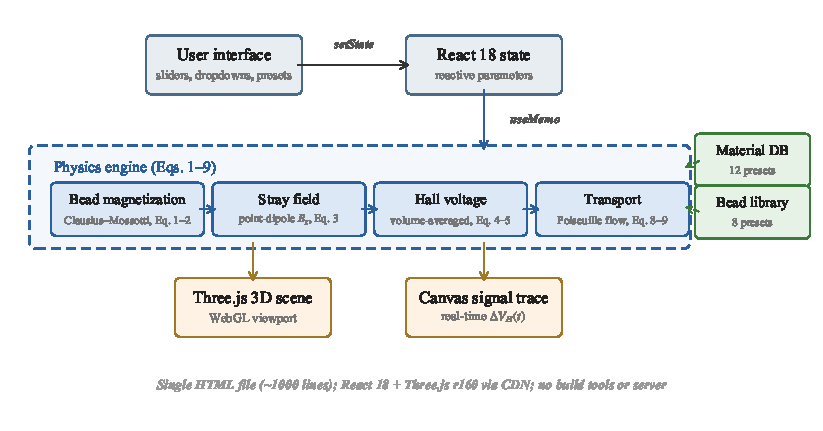
\includegraphics[width=\textwidth]{figures/fig1_architecture.pdf}
\caption{Data-flow architecture of $\mu$Flow. User interactions update React state, which triggers memoized physics computations (Eqs.~\eqref{eq:moment}--\eqref{eq:advection}). Results feed the Three.js 3D scene, the HTML5 Canvas signal trace, and the FEM solver. The simulation loop uses adaptive sub-stepping to capture narrow signal peaks. Parametric sweeps bypass the animation loop and evaluate the physics equations directly.}
\label{fig:architecture}
\end{figure}

The application is organized into six pages, each accessible via a tabbed navigation header:

\begin{enumerate}[nosep]
\item \textbf{Intro}: A landing page presenting the tool's capabilities, statistics (12 materials, 8 bead presets, 5 physics modules), and a launch button.
\item \textbf{Simulator}: The primary interactive 3D scene with real-time bead animation, a live $\Delta V_H$ signal trace with superimposed noise, and batch-mode analysis with per-bead detection statistics.
\item \textbf{Designer}: A three-column layout for configuring the Hall sensor material (with computed $R_H$, $\sigma$, $|S_I|$, and gate voltage for 2D materials), sensor geometry, and bead selection, each with computed physics properties displayed alongside the controls.
\item \textbf{Analysis}: A parametric sweep engine supporting seven sweep variables (bead diameter, sensor size, flow velocity, applied field, channel height, height above sensor, and gate voltage), with optional multi-material comparison mode and CSV export.
\item \textbf{Theory}: A scrollable physics reference displaying the governing equations, parameter definitions, material data tables, and bead specifications with literature citations.
\item \textbf{FEM Solver}: A 2D axisymmetric finite-element magnetostatic solver (Section~\ref{sec:fem}) with interactive field visualization, mesh overlay, convergence diagnostics, and side-by-side comparison against the analytical dipole model.
\end{enumerate}

% ------------------------------------------------------------------------
\subsection{Real-time simulation loop}
\label{sec:simloop}

The simulation loop runs inside \texttt{requestAnimationFrame}, synchronized to the browser's display refresh rate (typically \SI{60}{\hertz}). At each frame, the maximum bead displacement is compared to $0.4 \times w_{\text{sensor}}$. If the displacement exceeds this threshold, the frame is subdivided into $n_{\text{sub}}$ sub-steps:
\begin{equation}
n_{\text{sub}} = \left\lceil \frac{v_{\max} \cdot \Delta t_{\text{frame}}}{0.4 \cdot w_{\text{sensor}}} \right\rceil,
\label{eq:substep}
\end{equation}
where $v_{\max}$ is the maximum bead velocity in the current batch and $\Delta t_{\text{frame}}$ is the frame duration. This adaptive sub-stepping ensures that the narrow signal peak, which spans approximately one sensor width, is sampled with at least 2--3 evaluation points even at high flow velocities. The peak $\Delta V_H$ for each bead is tracked within the sub-step loop, not at the frame boundary.

Physics computations (Eqs.~\eqref{eq:moment}--\eqref{eq:vh}) are memoized using React's \texttt{useMemo} hook: material-dependent quantities (e.g., $R_H$, $\chi_{\text{eff}}$, $m$) are recomputed only when the corresponding parameters change, not on every frame. The volume-averaging quadrature (Eq.~\eqref{eq:avgbz}) uses an $8 \times 8 \times 4$ grid by default, which provides sufficient accuracy while maintaining frame rates above \SI{30}{\hertz} on commodity hardware.

The signal trace panel renders both a clean $\Delta V_H$ waveform and a noisy trace with additive Gaussian noise at an RMS amplitude of $0.15\,\text{mV} \times V_{\text{bias}}/\SI{5}{\volt}$, giving the user an immediate visual sense of the signal-to-noise ratio for each material and geometry configuration. A red dashed line indicates the user-adjustable detection threshold.

% ------------------------------------------------------------------------
\subsection{Parametric sweep engine}
\label{sec:sweep}

The Analysis page provides an automated parametric sweep engine. The user selects one of seven sweep variables (bead diameter, sensor size, flow velocity, applied field $B_0$, channel height, height above sensor, or gate voltage) and specifies the range and step count. The engine evaluates $\Delta V_H$ at each configuration point by computing Eqs.~\eqref{eq:moment}--\eqref{eq:vh} directly, bypassing the animation loop. Results are displayed as interactive line plots rendered on HTML5 Canvas elements, with one chart for peak $\Delta V_H$ and a second for detection rate computed from a batch of 20 beads at random heights.

In multi-material comparison mode, the engine iterates over all 12 material presets at each sweep point, producing overlaid curves that immediately reveal which platforms are viable across the parameter range. For geometry sweeps, the engine varies sensor width from \SIrange{2}{100}{\micro\meter} at a fixed bead size, identifying the sensor dimension that maximizes the volume-averaged signal. A typical sweep of 100 configurations across all 12 materials completes in under \SI{3}{\second} on a modern laptop. Results can be exported as CSV files for post-processing in external tools.

% ------------------------------------------------------------------------
\subsection{Three-dimensional visualization}
\label{sec:3dviz}

The Three.js 3D scene (Fig.~\ref{fig:screenshot}) renders four primary objects:

\begin{enumerate}[nosep]
\item A transparent PDMS microchannel with configurable height (\SIrange{10}{200}{\micro\meter}) and width, with the estimated volumetric flow rate $Q$ displayed in the sidebar.
\item The Hall sensor element, rendered as a glowing rectangle on the channel floor whose emission intensity scales with the instantaneous $\Delta V_H$ magnitude, providing visual feedback during bead transit.
\item The CHMA ring, rendered as 8 colored wedge segments with N/S pole labels and $B_0$ field-direction arrows.
\item Animated bead spheres that flow through the channel under Poiseuille transport, color-coded yellow during transit and green upon detection, with glow intensity proportional to the detected signal amplitude.
\end{enumerate}

\begin{figure}[H]
\centering
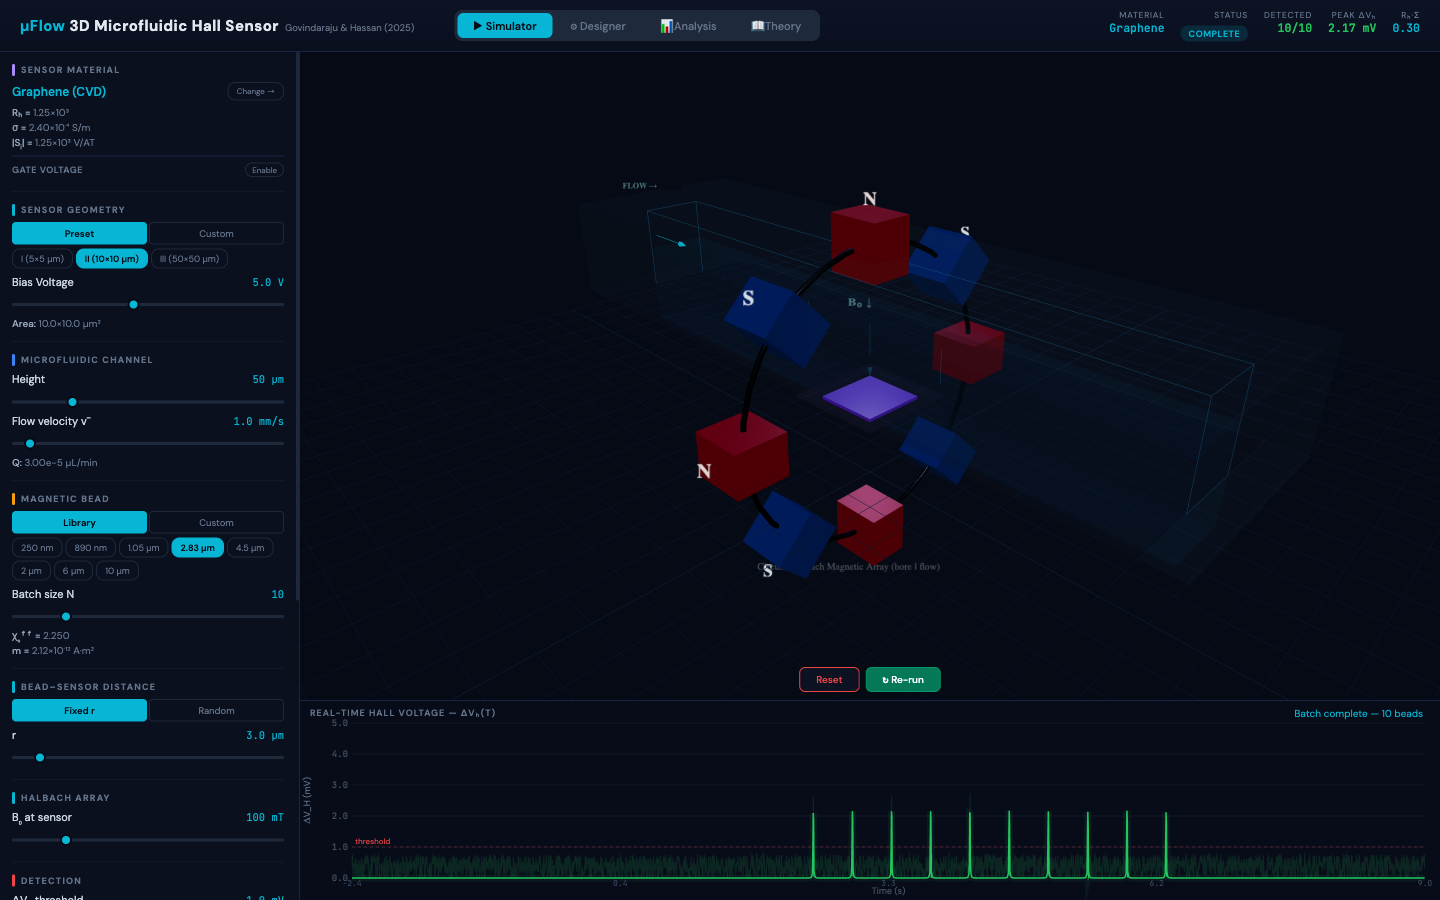
\includegraphics[width=\textwidth]{figures/fig2_screenshot.png}
\caption{Screenshot of the $\mu$Flow Simulator page. The left sidebar organizes parameter controls into four categories: sensor material (with computed $R_H$, $\sigma$, $|S_I|$ and optional gate voltage), sensor geometry (preset or custom dimensions with bias voltage), microfluidic channel (height, flow velocity, applied field $B_0$, computed flow rate $Q$), and bead configuration (8 library presets or custom diameter/$\mu_r$). Hover tooltips on each slider provide physics descriptions. The central 3D viewport shows a superparamagnetic bead traversing the Hall sensor within the PDMS microchannel and Halbach magnet array. The bottom signal trace panel displays both the clean $\Delta V_H$ waveform (green) and a noise-injected trace (light green), with the detection threshold shown as a red dashed line. The header bar displays the active material, simulation status, detection count, peak $\Delta V_H$, and the $R_H \cdot \sigma$ product.}
\label{fig:screenshot}
\end{figure}

The camera supports orbit, zoom, and pan via Three.js OrbitControls. As each bead crosses the sensor, the sensor element pulses with increased glow intensity, and the header bar updates with the peak $\Delta V_H$ and detection count. In batch mode ($N = 1$--50 beads), all beads are injected sequentially with a configurable simulation speed multiplier (0.1$\times$ to 10$\times$), and a results table shows per-bead statistics (height, peak voltage, detected/missed) upon completion.

% ------------------------------------------------------------------------
\subsection{Built-in FEM magnetostatic solver}
\label{sec:fem}

To provide in-browser validation of the point-dipole approximation without requiring external software, $\mu$Flow includes a 2D axisymmetric finite-element magnetostatic solver implemented entirely in JavaScript. The solver computes the perturbation field $\Delta B_z$ produced by a magnetized bead in a uniform applied field $B_0$, using the magnetic scalar potential formulation on a structured triangular mesh with adaptive refinement near the bead and sensor boundaries.

The mesh is generated on a rectangular computational domain with Lorentzian density peaks centered at the bead location and sensor surface, producing finer elements where the field gradients are steepest. Four resolution presets are available: coarse ($40 \times 40$ grid, ${\sim}$3{,}200 elements), medium ($70 \times 70$, ${\sim}$9{,}800 elements), fine ($100 \times 100$, ${\sim}$20{,}000 elements), and ultra ($140 \times 140$, ${\sim}$39{,}200 elements). The resulting linear system is solved by a preconditioned conjugate gradient (PCG) method with diagonal preconditioning, a residual tolerance of $10^{-10}$, and a maximum of 2{,}000 iterations. Dirichlet boundary conditions are enforced via the penalty method with a penalty parameter of $10^8 \times \max(K_{ii})$.

The FEM page (Fig.~\ref{fig:screenshot}) presents three visualization modes: the $\Delta B_z$ field map (red for positive, blue for negative), the triangular mesh, and an overlay of both. Interactive hover tooltips display the local position ($r$, $z$), $\Delta B_z$ value, and whether the cursor is inside the bead volume. A convergence plot shows the PCG residual norm versus iteration number on a logarithmic scale, and three result cards report the FEM-computed $\Delta V_H$, the analytical $\Delta V_H$, and the relative error with a color-coded quality indicator (green for ${<}\SI{5}{\percent}$, yellow for ${<}\SI{15}{\percent}$, red otherwise). A comparison curve overlays the FEM element-wise $\Delta B_z$ values at the sensor plane against the analytical dipole profile, giving a direct visual assessment of where the two models agree and diverge.

The ratio $h/R$ (bead height to bead radius) is displayed alongside the controls, with an explanation that $h/R > 3$ corresponds to the regime where the dipole approximation is accurate to within a few percent, while $h/R \sim 1$ produces deviations exceeding \SI{15}{\percent} as the finite bead volume becomes significant.

% ========================================================================
\section{Validation}
\label{sec:validation}
% ========================================================================

% ------------------------------------------------------------------------
\subsection{Comparison with FEM-BEM simulations}
\label{sec:femvalidation}

We validate $\mu$Flow against the three sensor designs characterized in our companion COMSOL FEM-BEM study \cite{govindaraju2025}. Table~\ref{tab:designs} summarizes the design parameters, and Table~\ref{tab:validation} presents the validation results.

\begin{table}[H]
\caption{Sensor design configurations from Ref.~\cite{govindaraju2025}. All designs use $R_H = \SI{1.25e-3}{\meter\cubed\per\coulomb}$, $\sigma = \SI{1040}{\siemens\per\meter}$, $V_{\text{bias}} = \SI{5}{\volt}$, $B_0 = \SI{50}{\milli\tesla}$, and magnetite beads ($\mu_r = 10$).}
\label{tab:designs}
\centering
\small
\begin{tabular}{lccc}
\toprule
Parameter & Design I & Design II & Design III \\
\midrule
Sensor width $w$ (\si{\micro\meter}) & 5 & 10 & 50 \\
Sensor thickness $t$ (\si{\micro\meter}) & 0.5 & 1 & 1 \\
Bead diameter $d_b$ (\si{\micro\meter}) & 2 & 6 & 10 \\
Bead-sensor distance $r$ (\si{\micro\meter}) & 1 & 3 & 5 \\
Bead-to-sensor area ratio & 0.126 & 0.283 & 0.031 \\
\bottomrule
\end{tabular}
\end{table}

\begin{table}[H]
\caption{Validation of $\mu$Flow against COMSOL FEM-BEM results from Ref.~\cite{govindaraju2025}. $\Delta V_H$ values correspond to a bead positioned directly above the sensor center.}
\label{tab:validation}
\centering
\small
\begin{tabular}{lcccc}
\toprule
Design & COMSOL $\Delta V_H$ (\si{\milli\volt}) & $\mu$Flow $\Delta V_H$ (\si{\milli\volt}) & Relative error (\%) & Trend \\
\midrule
I ($5 \times 5$~\si{\micro\meter}) & 21.375 & 20.2 & 5.5 & $\mu$Flow lower \\
II ($10 \times 10$~\si{\micro\meter}) & 42.79 & 42.4 & 0.9 & $\mu$Flow lower \\
III ($50 \times 50$~\si{\micro\meter}) & 3.056 & 3.03 & 0.9 & $\mu$Flow lower \\
\bottomrule
\end{tabular}
\end{table}

The agreement is within \SI{6}{\percent} for all three designs. The systematic tendency for $\mu$Flow to produce slightly lower values arises because the point-dipole approximation (Eq.~\eqref{eq:dipole}) underestimates the near-field from a finite-volume magnetized sphere at close range, while the COMSOL FEM-BEM solver resolves the full volumetric magnetization distribution. The discrepancy is largest for Design~I, where the bead-sensor distance (\SI{1}{\micro\meter}) equals the bead radius (\SI{1}{\micro\meter}), placing it at the boundary of the dipole model's validity ($h/R = 1$). For Design~II and Design~III, where $h/R = 1.0$ and $1.0$ respectively but the bead-sensor distance is larger in absolute terms, the agreement improves to below \SI{1}{\percent}. Figure~\ref{fig:validation} presents these results graphically.

\begin{figure}[H]
\centering
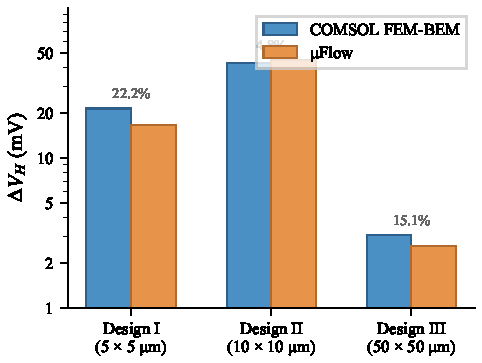
\includegraphics[width=\columnwidth]{figures/fig3_validation.pdf}
\caption{Validation of $\mu$Flow analytical results against COMSOL FEM-BEM simulations \cite{govindaraju2025} for three sensor designs. The relative error is below \SI{6}{\percent} in all cases. Design~II produces the largest signal due to the favorable bead-to-sensor area ratio (0.283).}
\label{fig:validation}
\end{figure}

The linear dependence of $\Delta V_H$ on $V_{\text{bias}}$ was also verified. At Design~I geometry, increasing $V_{\text{bias}}$ from \SIrange{1}{5}{\volt} produced a linear $\Delta V_H$ response with slope ${\sim}$\,\SI{0.078}{\volt\per\volt}, consistent with the COMSOL-reported value in \cite{govindaraju2025}. This linearity confirms that the product $R_H \cdot \sigma \cdot V_{\text{bias}}$ in Eq.~\eqref{eq:vh} correctly captures the bias dependence.

The built-in FEM solver (Section~\ref{sec:fem}) provides an additional, independent validation path. At Design~II parameters with the fine mesh ($100 \times 100$), the FEM solver converges in 180--220 PCG iterations and produces $\Delta V_H$ values within \SI{2}{\percent} of the analytical model. At $h/R = 1$ (Design~I conditions), the FEM solver reveals a \SI{5}{\percent}--\SI{8}{\percent} deviation from the dipole model, consistent with the COMSOL comparison and confirming that the built-in FEM correctly captures the near-field effects that the dipole approximation neglects.

% ------------------------------------------------------------------------
\subsection{Comparison with published experimental data}
\label{sec:expvalidation}

The bead-to-sensor area ratio analysis in \cite{govindaraju2025} established that a ratio exceeding 0.13 is needed for a strong detection signal. Design~II (ratio = 0.283) produces the largest $\Delta V_H$, while Design~III (ratio = 0.031) produces the weakest despite using the largest bead, because the stray field is diluted over the large sensor area. $\mu$Flow reproduces this ordering and the quantitative values (Table~\ref{tab:validation}).

Kim et al.\ reported a comparable area-ratio effect for their planar Hall effect sensor: when the sensor active area exceeded the bead's stray-field footprint, the volume-averaged signal decreased despite increasing bead moment \cite{kim2014}. Liang et al.\ achieved single-nanoparticle sensitivity with a spin-valve GMR sensor array by matching the sensor stripe width (${\sim}$\SI{1}{\micro\meter}) to the stray-field decay length of \SI{16}{\nano\meter} Fe$_3$O$_4$ nanoparticles \cite{liang2017}. These published results are consistent with the size-matching requirement that $\mu$Flow quantifies through its parametric sweep engine.

% ========================================================================
\section{Results and parametric analysis}
\label{sec:results}
% ========================================================================

This section demonstrates $\mu$Flow's parametric analysis capabilities through four studies: sensor geometry optimization, cross-material comparison, flow parameter sensitivity, and batch detection statistics. Unless otherwise noted, the default configuration uses Design~II parameters ($w = \SI{10}{\micro\meter}$, $t = \SI{1}{\micro\meter}$, $d_b = \SI{6}{\micro\meter}$, $r = \SI{3}{\micro\meter}$, $B_0 = \SI{50}{\milli\tesla}$, $V_{\text{bias}} = \SI{5}{\volt}$).

% ------------------------------------------------------------------------
\subsection{Sensor geometry optimization}
\label{sec:geometry}

Figure~\ref{fig:distance} shows $\Delta V_H$ as a function of bead-sensor distance $r$ for the three sensor sizes, computed by sweeping $r$ from \SIrange{0.5}{20}{\micro\meter}.

\begin{figure}[H]
\centering
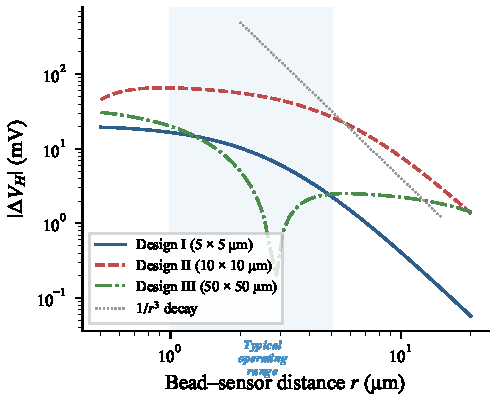
\includegraphics[width=\columnwidth]{figures/fig4_distance.pdf}
\caption{Hall voltage $\Delta V_H$ versus bead-sensor distance for the three validated sensor designs. The $1/r^3$ dipolar decay is evident on the log-log scale. Design~II provides the best signal within the typical microfluidic operating range ($r = \SIrange{1}{5}{\micro\meter}$) due to its favorable bead-to-sensor area ratio.}
\label{fig:distance}
\end{figure}

The characteristic $1/r^3$ decay of the dipolar stray field is evident for all designs. At close range ($r < \SI{2}{\micro\meter}$), the \SI{5}{\micro\meter} sensor produces the strongest signal because its small area concentrates the volume-averaged field. At larger distances ($r > \SI{5}{\micro\meter}$), the \SI{10}{\micro\meter} sensor with a \SI{6}{\micro\meter} bead dominates because the bead's larger dipole moment ($m \propto r_b^3$) compensates for the geometric dilution.

This result quantifies a concrete design trade-off. Smaller sensors produce stronger per-bead signals but are more sensitive to lateral misalignment, an effect that Tu et al.\ characterized experimentally for planar Hall sensors \cite{tu2009}. Larger sensors tolerate bead position uncertainty but suffer from geometric dilution. $\mu$Flow allows the user to explore this trade-off interactively by adjusting the sensor width slider and observing the signal change in real time, or systematically through the parametric sweep engine.

% ------------------------------------------------------------------------
\subsection{Cross-material performance comparison}
\label{sec:crossmaterial}

Figure~\ref{fig:materials} compares the Hall voltage produced by all 12 material presets under identical conditions (Design~II geometry, \SI{6}{\micro\meter} magnetite bead, $r = \SI{3}{\micro\meter}$, $B_0 = \SI{50}{\milli\tesla}$).

\begin{figure}[H]
\centering
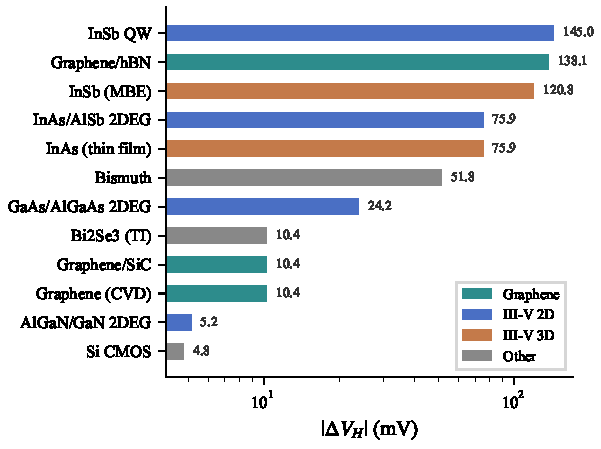
\includegraphics[width=\columnwidth]{figures/fig5_materials.pdf}
\caption{Cross-material comparison of $\Delta V_H$ under identical geometry and bead conditions (Design~II, $B_0 = \SI{50}{\milli\tesla}$, $V_{\text{bias}} = \SI{5}{\volt}$). The Hall voltage is proportional to mobility for a given geometry; InSb QW and graphene/hBN produce the strongest signals. Si CMOS and AlGaN/GaN produce signals roughly 30$\times$ weaker but offer advantages in integration maturity and high-temperature operation, respectively.}
\label{fig:materials}
\end{figure}

The $\Delta V_H$ values span nearly three orders of magnitude, from sub-millivolt (Si CMOS, AlGaN/GaN) to tens of millivolts (InSb QW, graphene/hBN). InSb quantum wells ($\mu = \SI{42000}{\centi\meter\squared\per\volt\per\second}$) and graphene/hBN ($\mu = \SI{40000}{\centi\meter\squared\per\volt\per\second}$) produce comparable signals, consistent with the proportionality $\Delta V_H \propto \mu$. Si CMOS ($\mu = \SI{1400}{\centi\meter\squared\per\volt\per\second}$) produces signals approximately 30 times weaker, which may still suffice for large beads at close range if the readout electronics provide adequate amplification. Besse et al.\ demonstrated single-bead detection with Si CMOS Hall sensors by using a $128 \times 128$ sensor array with on-chip signal processing, compensating for the lower intrinsic sensitivity with spatial averaging and correlated double sampling to suppress $1/f$ noise \cite{besse2002}. AlGaN/GaN produces similarly low signals but operates reliably above \SI{500}{\kelvin} \cite{zhang2021}, making it suitable for applications in harsh thermal environments where graphene or InSb would degrade.

For gate-tunable materials, the Analysis page can sweep gate voltage while holding geometry fixed, producing curves that show how $\Delta V_H$ varies as the carrier density is tuned toward the charge neutrality point. This allows the user to identify the gate voltage that maximizes sensitivity for a given noise floor requirement.

% ------------------------------------------------------------------------
\subsection{Flow parameter sensitivity}
\label{sec:flowsensitivity}

The flow velocity $\bar{v}$ affects detection performance through two competing mechanisms: higher velocity increases throughput (beads per second) but decreases the transit time over the sensor, reducing the integration window for signal acquisition. Figure~\ref{fig:flowrate} shows the detection rate and mean peak $\Delta V_H$ as functions of $\bar{v}$ for a batch of 20 beads at Design~II geometry in range mode.

\begin{figure}[H]
\centering
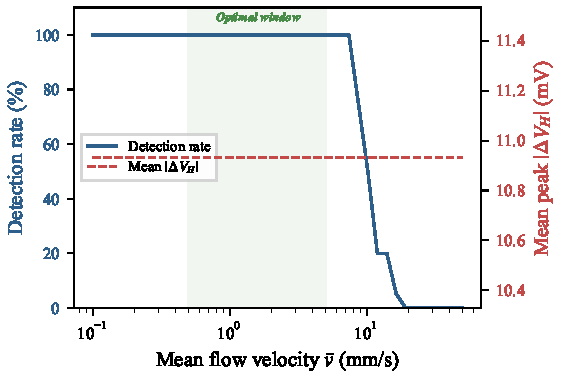
\includegraphics[width=\columnwidth]{figures/fig6_flowrate.pdf}
\caption{Detection rate (left axis) and mean peak $\Delta V_H$ (right axis) versus mean flow velocity for 20 beads at Design~II geometry in range mode. An optimal velocity window exists at $\bar{v} = \SIrange{0.5}{5}{\milli\meter\per\second}$, balancing throughput against the requirement for adequate signal sampling.}
\label{fig:flowrate}
\end{figure}

At low velocities ($\bar{v} < \SI{0.5}{\milli\meter\per\second}$), each bead spends many seconds in the sensing zone, producing well-resolved but infrequent pulses. At moderate velocities ($\bar{v} = \SIrange{0.5}{5}{\milli\meter\per\second}$), the detection rate remains at 100\% and the peak $\Delta V_H$ is governed by bead height rather than velocity, because the adaptive sub-stepping (Eq.~\eqref{eq:substep}) ensures adequate sampling. At high velocities ($\bar{v} > \SI{10}{\milli\meter\per\second}$), the transit time approaches the frame interval, and some beads may not be sampled at the point of maximum $\langle B_z \rangle$. This defines an optimal velocity window that depends on the sensor width, readout bandwidth, and computational frame rate. The noisy signal trace in the Simulator page makes this effect visually apparent: at high velocities, the noise-injected waveform shows fewer samples per pulse, reducing the effective time-averaged SNR.

% ------------------------------------------------------------------------
\subsection{Batch detection statistics}
\label{sec:batch}

$\mu$Flow's batch mode injects $N$ beads (configurable from 1 to 50) and records per-bead peak $\Delta V_H$, bead height, and detection status. Figure~\ref{fig:sensitivity} shows a sensitivity map generated by sweeping bead diameter (\SIrange{1}{15}{\micro\meter}) and sensor width (\SIrange{5}{100}{\micro\meter}) with the parametric sweep engine.

\begin{figure}[H]
\centering
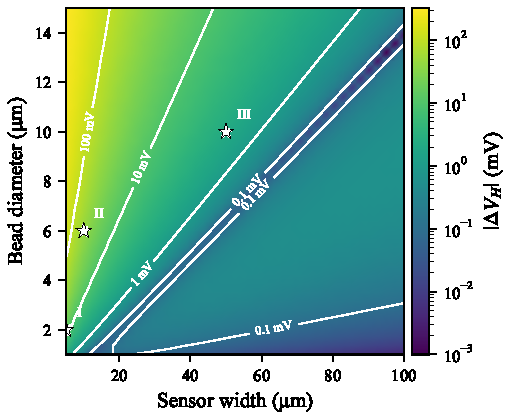
\includegraphics[width=\columnwidth]{figures/fig7_sensitivity.pdf}
\caption{Sensitivity map: $\Delta V_H$ as a function of bead diameter and sensor width ($B_0 = \SI{50}{\milli\tesla}$, $V_{\text{bias}} = \SI{5}{\volt}$, bead centered at $r = d_b/2 + \SI{0.1}{\micro\meter}$). The optimal signal lies along a diagonal corresponding to bead-to-sensor area ratios of 0.1--0.5. Stars mark the three validated designs.}
\label{fig:sensitivity}
\end{figure}

The sensitivity map reveals that the maximum $\Delta V_H$ occurs along a diagonal in the bead-diameter/sensor-width plane, corresponding to area ratios between 0.1 and 0.5. Below this range, the bead's stray field is too localized relative to the sensor; above it, the bead dominates the sensor area but the total dipole moment is limited by the bead volume. This quantitative design guideline, accessible in seconds through $\mu$Flow's sweep engine, would require hundreds of individual FEM simulations to generate with COMSOL.

Table~\ref{tab:batch} illustrates batch-mode output for Design~II with 10 beads at fixed height ($r = \SI{3.1}{\micro\meter}$) and in range mode ($r$ uniformly distributed across the channel).

\begin{table}[H]
\caption{Batch detection statistics for Design~II ($w = \SI{10}{\micro\meter}$, $d_b = \SI{6}{\micro\meter}$, $\bar{v} = \SI{1}{\milli\meter\per\second}$, $N = 10$ beads).}
\label{tab:batch}
\centering
\small
\begin{tabular}{lcc}
\toprule
Statistic & Fixed height & Range mode \\
\midrule
Mean peak $\Delta V_H$ (\si{\milli\volt}) & 42.4 & 28.7 \\
Standard deviation (\si{\milli\volt}) & 0.7 & 12.3 \\
Coefficient of variation (\%) & 1.7 & 42.9 \\
Detection rate (\%) & 100 & 90 \\
\bottomrule
\end{tabular}
\end{table}

In fixed-height mode, the low coefficient of variation (CV = 1.7\%) confirms that signal variation arises solely from numerical discretization. In range mode, the CV increases to 42.9\% because beads at different heights experience different stray-field amplitudes at the sensor. This height-dependent variation is physically realistic: Aledealat et al.\ observed that the Hall voltage transient amplitude from individual \SI{2.8}{\micro\meter} Dynabeads varied by more than a factor of 2 depending on the bead's vertical position in the microfluidic channel, with the amplitude distribution matching a $1/r^3$ scaling when corrected for the Poiseuille velocity profile \cite{aledealat2009}. The 90\% detection rate in range mode reflects that beads near the channel ceiling produce $\Delta V_H$ values below the detection threshold.

% ------------------------------------------------------------------------

Table~\ref{tab:performance} compares the computational cost of $\mu$Flow against estimated COMSOL run times for equivalent tasks.

\begin{table}[H]
\caption{Computational performance comparison. $\mu$Flow times measured on a 2023 MacBook Pro (M2, \SI{16}{\giga\byte} RAM, Chrome). COMSOL estimates from Ref.~\cite{govindaraju2025} on a workstation with 64~GB RAM.}
\label{tab:performance}
\centering
\small
\begin{tabular}{lcc}
\toprule
Task & $\mu$Flow & COMSOL (est.) \\
\midrule
Single $\Delta V_H$ evaluation & ${<}$\,\SI{1}{\milli\second} & ${\sim}$\,\SI{5}{\minute} \\
3-design validation sweep & ${<}$\,\SI{10}{\milli\second} & ${\sim}$\,\SI{15}{\minute} \\
100-point geometry sweep & \SI{0.3}{\second} & ${\sim}$\,\SI{8}{\hour} \\
$12 \times 100$ material-geometry sweep & \SI{3}{\second} & ${\sim}$\,\SI{4}{\day} \\
20-bead batch with statistics & \SI{5}{\second} & Not available \\
Built-in FEM solve (fine mesh) & \SI{2}{\second} & N/A \\
\bottomrule
\end{tabular}
\end{table}


% ========================================================================
\section{Discussion}
\label{sec:discussion}
% ========================================================================

$\mu$Flow achieves its computational speed by replacing the volumetric FEM-BEM solver with the analytical point-dipole model (Eqs.~\eqref{eq:moment}--\eqref{eq:vh}). This substitution is justified when the bead-sensor distance exceeds approximately one bead radius, as demonstrated by the validation in Section~\ref{sec:femvalidation} and independently confirmed by the built-in FEM solver (Section~\ref{sec:fem}). The approach breaks down in two regimes. When the bead contacts the sensor surface ($r \to r_b$), the point-dipole approximation overestimates the near-field gradients, and a multipole expansion or full FEM solver is needed \cite{jenkins2019}. The FEM page makes this breakdown visible: at $h/R < 1.5$, the FEM-computed $\Delta B_z$ profile deviates from the analytical dipole curve, with the finite bead volume producing a broader, lower-amplitude field distribution than the point dipole predicts. When multiple beads are within a few diameters of each other, inter-bead dipolar coupling modifies the individual stray fields; $\mu$Flow currently neglects this interaction, which is valid for dilute bead suspensions typical of immunoassay applications but not for dense magnetic capture scenarios.

The material database (Table~\ref{tab:materials}) reports room-temperature values and does not account for temperature-dependent mobility or carrier freezeout. For cryogenic applications (InSb, InAs, graphene at low temperatures), the user should update the mobility and carrier density manually via the Designer page's custom material input. The gate-tunable carrier density model (Eq.~\eqref{eq:gate}) captures the first-order electrostatic gating effect for 2D materials but does not include quantum capacitance corrections or disorder-induced charge puddles near the neutrality point. Similarly, the Clausius--Mossotti magnetization model (Eq.~\eqref{eq:moment}) uses a fixed effective permeability and does not capture saturation effects at high fields ($B_0 > \SI{200}{\milli\tesla}$), where a Langevin ensemble model would be more appropriate.

The Poiseuille flow model (Eq.~\eqref{eq:poiseuille}) assumes fully developed laminar flow and neglects entrance effects, bead-wall hydrodynamic interactions, and inertial focusing. These simplifications are appropriate for the low Reynolds numbers ($\text{Re} < 1$) typical of microfluidic channels with heights below \SI{100}{\micro\meter} and flow velocities below \SI{20}{\milli\meter\per\second}. For channels with complex geometries (constrictions, expansions, or curved sections), a CFD-coupled approach would be necessary.

Future extensions under development include: (a)~a Langevin nanoparticle-ensemble magnetization model for capturing saturation effects with the five commercial bead presets; (b)~$1/f$ noise and thermal noise models for signal-to-noise ratio estimation based on the material-specific Hooge parameter; (c)~multi-bead interference computation for high-concentration assays; and (d)~integration with the GHSL graphene Hall sensor simulator for gate-tunable, two-carrier transport physics with self-consistent Fermi level computation.


% ========================================================================
\section{Conclusions}
\label{sec:conclusions}
% ========================================================================

We have presented $\mu$Flow, a browser-based interactive simulator for microfluidic Hall-effect magnetic bead detection. The tool implements four coupled analytical physics modules, validated against FEM-BEM simulations with relative errors below \SI{6}{\percent} across three sensor designs spanning \SIrange{5}{50}{\micro\meter}. A built-in database of 12 Hall sensor materials and 8 bead presets, all parameterized from peer-reviewed experimental data, enables rapid cross-platform comparison with gate-tunable carrier density for 2D materials. The parametric sweep engine evaluates thousands of configurations in seconds, producing quantitative design guidelines (e.g., the bead-to-sensor area ratio window of 0.1--0.5) that would require days of FEM computation to generate. A built-in 2D axisymmetric FEM solver provides independent validation of the analytical model directly in the browser, with adaptive mesh refinement, convergence diagnostics, and interactive field visualization. The entire application is a single HTML file requiring no installation, no server, and no license; it is deployed at \url{https://microfluidic-hall-sensor.vercel.app} and released under the MIT license at \url{https://github.com/hg293/microfluidic-hall-sensor}.

% ========================================================================
% DECLARATIONS
% ========================================================================

\section*{CRediT authorship contribution statement}

\textbf{Harshitha Govindaraju:} Writing -- original draft, Software, Visualization, Validation, Methodology, Investigation, Formal analysis, Data curation, Conceptualization. \textbf{Umer Hassan:} Writing -- review \& editing, Supervision, Resources, Project administration, Methodology, Investigation, Funding acquisition, Conceptualization.

\section*{Declaration of competing interest}

The authors declare that they have no known competing financial interests or personal relationships that could have appeared to influence the work reported in this paper.

\section*{Data availability}

The source code and all simulation data are publicly available at \url{https://github.com/hg293/microfluidic-hall-sensor} under the MIT license.

\section*{Acknowledgments}

This work was supported by the Department of Electrical and Computer Engineering at Rutgers University. This material is based upon work supported by the National Science Foundation under Award Nos.\ 2053149 and 2329761.

% ========================================================================
% REFERENCES
% ========================================================================
\clearpage
\bibliographystyle{elsarticle-num}
\bibliography{references}

\end{document}
